\documentclass{article}
\usepackage{nips13submit_e,times}
\usepackage{hyperref}
\usepackage{url}
\usepackage{subcaption}       % \begin{subfigure}
\usepackage{graphicx}

\title{User Interface Parsing}
\author{
Calvin Loncaric\\
Department of Computer Science and Engineering\\
University of Washington\\
Seattle, WA\\
\texttt{loncaric@cs.washington.edu}\\
\url{https://homes.cs.washington.edu/\~loncaric}}
\date{June 8, 2015}

\newcommand{\fix}{\marginpar{FIX}}
\newcommand{\new}{\marginpar{NEW}}

\nipsfinalcopy % Uncomment for camera-ready version

% Useful tips:
%
%    \verb+text+      verbatim text
%
% \begin{table}[t]
% \caption{Sample table title}
% \label{sample-table}
% \begin{center}
% \begin{tabular}{ll}
% \multicolumn{1}{c}{\bf PART}  &\multicolumn{1}{c}{\bf DESCRIPTION}
% \\ \hline \\
% Dendrite         &Input terminal \\
% Axon             &Output terminal \\
% Soma             &Cell body (contains cell nucleus) \\
% \end{tabular}
% \end{center}
% \end{table}
%
% \begin{figure}[h]
% \begin{center}
% %\framebox[4.0in]{$\;$}
% \fbox{\rule[-.5cm]{0cm}{4cm} \rule[-.5cm]{4cm}{0cm}}
% \end{center}
% \caption{Sample figure caption.}
% \end{figure}

\begin{document}
\maketitle

\begin{abstract}
While easy to describe on paper, user interfaces are still tedious to construct
on a computer. Many programmer work hours are wasted translating design sketches
into code. There is a need for a tool which can automatically translate hand-%
drawn sketches into code without programmer assistance. In this work I describe
a possible approach to this problem using computer vision techniques. All code
and artifacts for this work are available online%
\footnote{\url{https://github.com/Calvin-L/ui-parser}}.
\end{abstract}

\section{Related Work}

The task of parsing a sketch of a user interface can be broken down into three
parts:
\begin{enumerate}
\item what UI elements are present? (e.g. text, images, forms, spacers)
\item what are the layout constraints? (e.g. widths, heights, paddings,
    containment relationships)
\item what is the simplest layout which contains all the elements and satisfies
    the given constraints?
\end{enumerate}

Thus, three bodies of work relate directly to this project: sketch recognition,
handwriting recognition, and constraint solvers.

Sketch recognition techniques have been developed for several domains, including
circuit diagrams and flowcharts. There have ben been efforts to simplify the
task, allowing experts to declaratively write descriptions of objects and have
the computer parse them from sketches \cite{ShapeDescriptions2004,
SketchREAD2007}.

While promising, these sketch recognition engines alone are not able to
effectively use context information (i.e. nearby drawing elements) to improve
accuracy. The approach I describe in \autoref{sec:element-detection} relies
almost exclusively on observations of surrounding elements in order to parse the
sketch.

Accurate handwriting recognition is needed in order to parse text and
annotations in user interface sketches. Handwriting recognition is an
extensively studied problem in computer vision \cite{HandwritingRecSurvey2000},
yet there do not seem to be any freely available off-the-shelf tools for finding
and recognizing sparse text on sketches.

In this work I used Google's Tesseract library \cite{Tesseract}, but Tesseract
is optimized for book text and the quality of the tool could be vastly improved
with a better handwriting recognition algorithm. More details are written in
\autoref{sec:constraint-formation}.

Microsoft's Z3 \cite{Z32008} is one of the most efficient and widely-used
constraint solvers. Z3 is a very general solver and can solve systems of
constraints involving booleans, integers, real numbers, arrays, and other
high-level types. Given the complex, hierarchical nature of user interfaces,
however, Z3 is a poor choice. There exist several constraint solvers
specifically for the domain of user interfaces; SkyBlue \cite{SkyBlue1994} is
one notable example. Researchers have also studied constraint-based layout
specifications for the web \cite{ConstraintsForTheWeb1997}.

In this work, I do not intend to solve the problem of layout generation from
constraints. The algorithm currently implemented in the tool uses a set of
handwritten heuristics (described in \autoref{sec:layout-gen}) and could
persumably be replaced with a smarter approach given more engineering time.

\section{Framework}

This section describes the actual operation of the tool. The input is a sketch
(such as one from \autoref{fig:sample-inputs}) and the output is a user
interface in the form of an HTML page (as in \autoref{fig:sample-outputs}).

\subsection{Element Detection}
\label{sec:element-detection}

\subsection{Constraint Formation}
\label{sec:constraint-formation}

\subsection{Layout Generation}
\label{sec:layout-gen}

The layout generation engine is not a major contribution of this work, so it
will not be discussed in any great detail.

At a high level, the layout generation engine works by recursively identifying
all the roots of the layout (i.e. elements which are not constrained to be
contained within another element). Once the roots are found, the algorithm
groups elements by which root they belong to and recurses. Elements belonging
to more than one root are arbitrarily assigned to one.

For each root, the algorithm then finds a constraint for top, left, bottom, and
right margins; width; and height. Additional or conflicting constraints are
discarded. Any missing values are filled in by estimating distances from the
original sketch. The resulting values are written out as CSS. Random background
colors are chosen for each UI element to make reading the layout easier.

\section{Results and Discussion}

\begin{figure}[h]
\begin{center}
    \begin{subfigure}[b]{0.3\textwidth}
        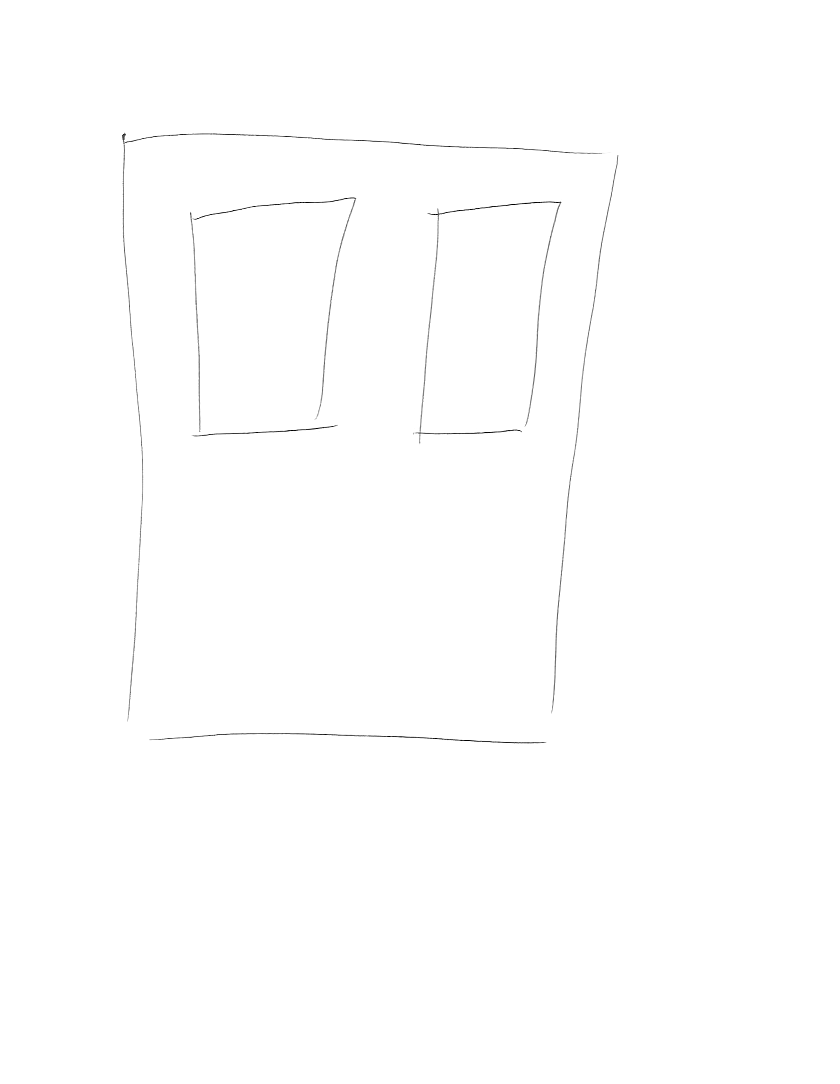
\includegraphics[width=\textwidth]{../examples/scan-01.png}
        \caption{\texttt{scan-01.png}}
    \end{subfigure}
    \begin{subfigure}[b]{0.3\textwidth}
        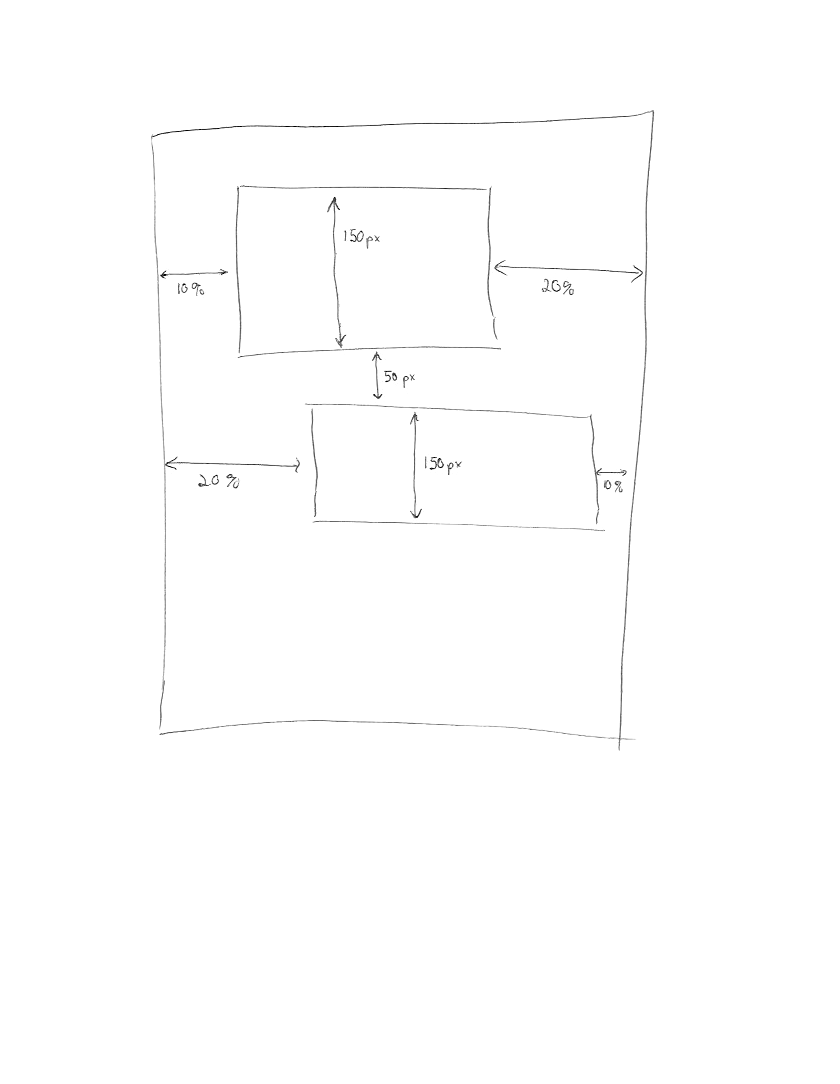
\includegraphics[width=\textwidth]{../examples/scan-04.png}
        \caption{\texttt{scan-04.png}}
    \end{subfigure}
    \begin{subfigure}[b]{0.3\textwidth}
        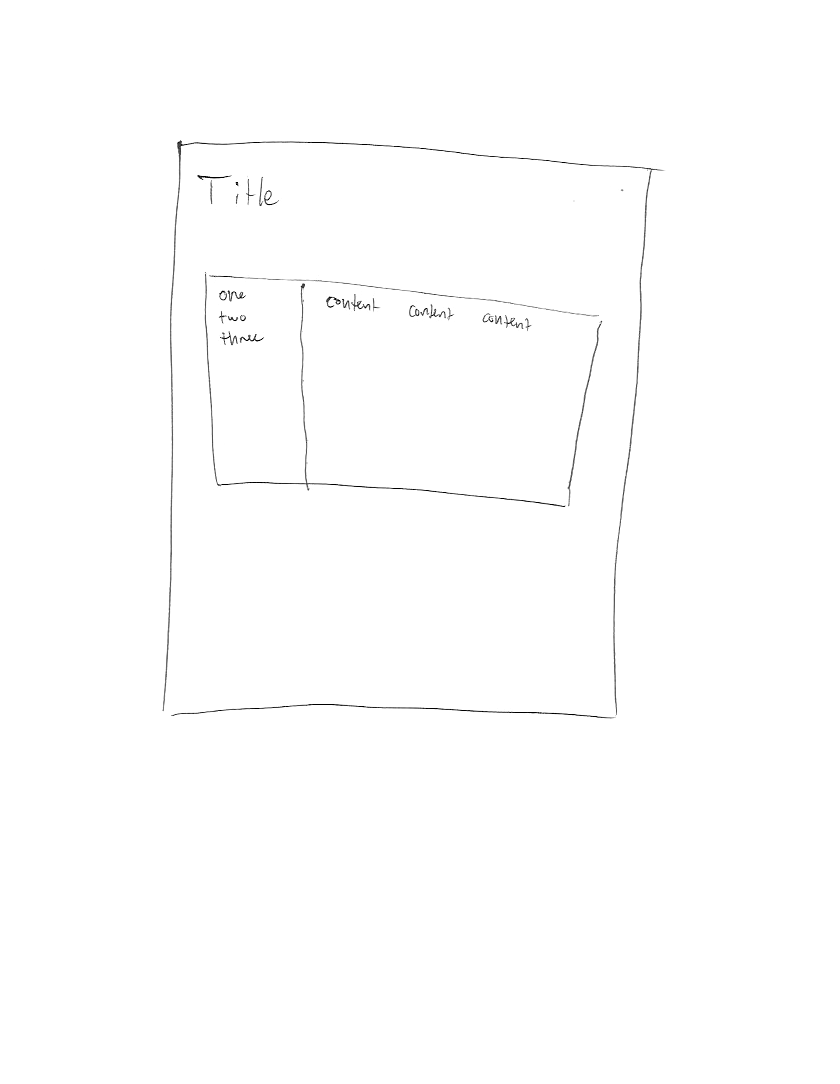
\includegraphics[width=\textwidth]{../examples/scan-08.png}
        \caption{\texttt{scan-08.png}}
    \end{subfigure}
\end{center}
\caption{A few sample inputs. The sketches ranged from simple (just boxes, no
    explicit constraints) to moderate (just boxes with explicit constraints) to
    complex (numerous UI elements including text, images, and tables).}
\label{fig:sample-inputs}
\end{figure}

\begin{figure}[h]
\begin{center}
    \begin{subfigure}[b]{0.3\textwidth}
        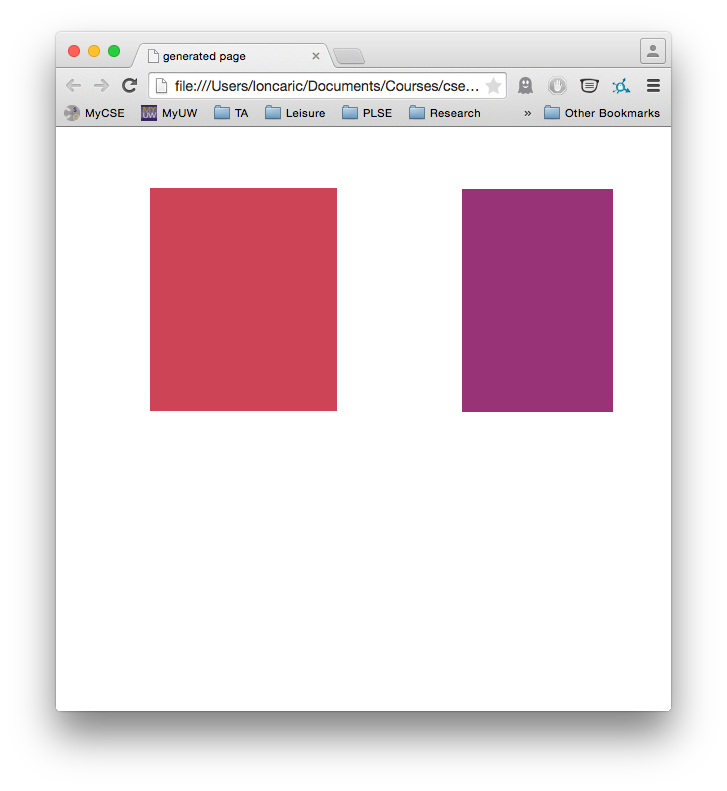
\includegraphics[width=\textwidth]{scan-01-output.png}
        \caption{\texttt{scan-01.png}}
    \end{subfigure}
    \begin{subfigure}[b]{0.3\textwidth}
        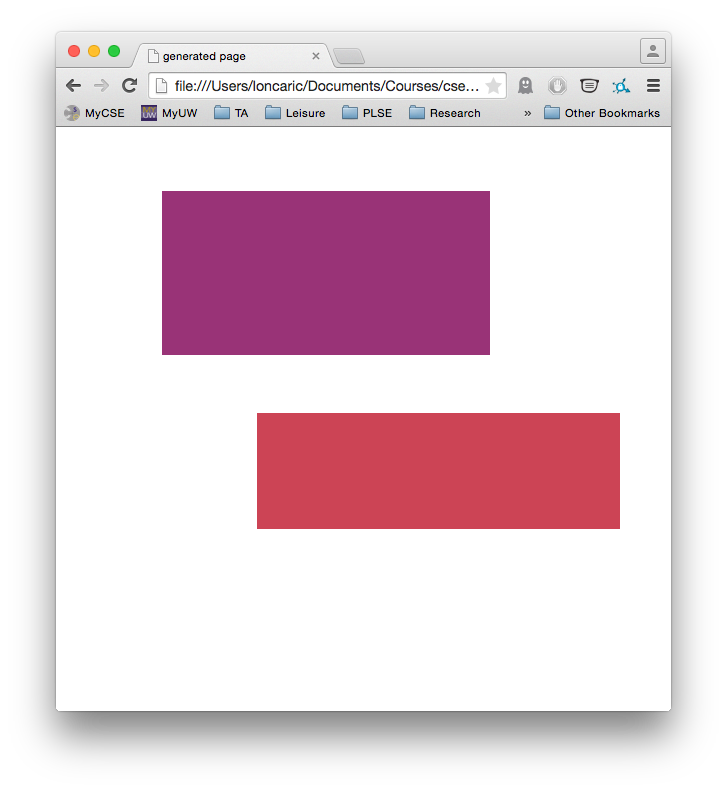
\includegraphics[width=\textwidth]{scan-04-output.png}
        \caption{\texttt{scan-04.png}}
    \end{subfigure}
    \begin{subfigure}[b]{0.3\textwidth}
        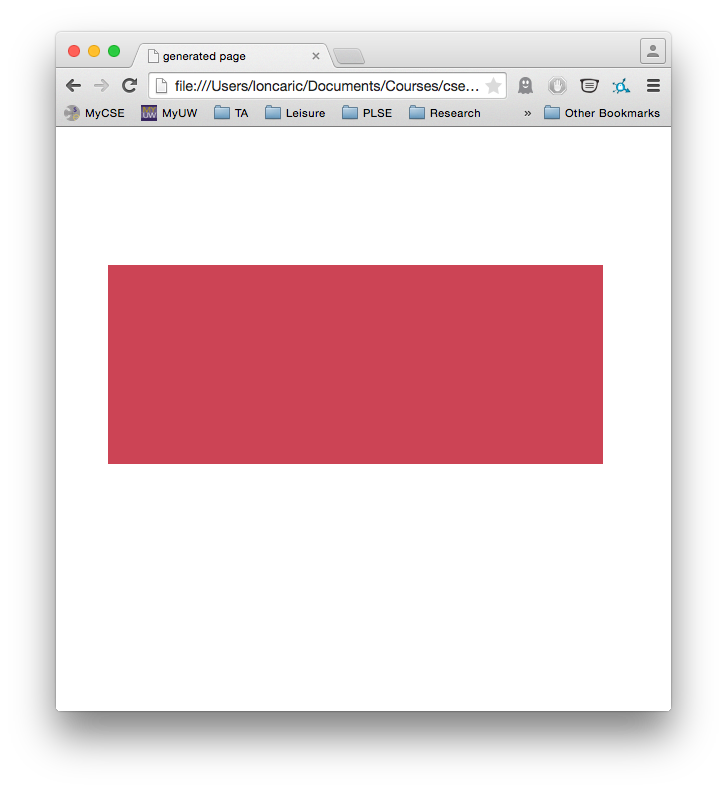
\includegraphics[width=\textwidth]{scan-08-output.png}
        \caption{\texttt{scan-08.png}}
    \end{subfigure}
\end{center}
\caption{Output screenshots for the sample images in
\autoref{fig:sample-inputs}.}
\label{fig:sample-outputs}
\end{figure}

\begin{table}[h]
\begin{center}
\input{benchmark.tex}
\end{center}
\caption{Timings and output qualities for each of the example inputs. The
    timings were collected on a 2012 MacBook Pro with a 2-core 2.5 GHz Intel
    Core i5 processor and 8 Gb of RAM. The output quality is a qualitative
    measure manually assessed by the author for each file. ``Perfect'' means
    that the output layout perfectly matched the input sketch. ``Good'' means
    that all major layout elements were identified, but some measurements were
    off. ``Bad'' means that some layout elements were missing and/or many
    measurements were off. ``Fail'' means that the output did not resemble the
    input sketch.}
\label{tbl:benchmarks}
\end{table}

At the beginning of the project I drew and scanned 13 sample layouts. Results
for each one are summarized in \autoref{tbl:benchmarks}. To give some indication
of what these sample inputs look like, a few selected images are shown in
\autoref{fig:sample-inputs}, with corresponding outputs in
\autoref{fig:sample-outputs}.

While the tool performs very well on early examples involving only boxes and
constraints, I did not have time to complete the project and implement parsing
for more complex elements (e.g. text, images, or tables). The presence of more
complex elements is what causes scores of ``bad'' and ``fail'' on many inputs.
As a general rule, the tool performs perfectly on inputs with just boxes (it
guesses at constraints fairly well), but due to limitations in the handwriting
recognition code it cannot reliably understand constraints, earning a score of
``good'' on those examples.

\section{Conclusion}

\bibliography{bibliography}{}
\bibliographystyle{unsrt}

\end{document}
